\section{使用 \tkzname{alterqcm} 和 \tkzname{tkz-tab} 宏包的示例}

\begin{alterqcm}[lq=110mm]

\AQmessage{图 1 显示了定义在 $[0, +\infty)$ 上的函数 $f$ 的图像，图 2 显示了 $f$ 在 $[0, +\infty)$ 上的一个原函数的图像。

\begin{center}
 \begin{tikzpicture}[xscale=2.25,yscale=1]
   \tkzFnInit[xmin=-2,xmax=3,ymin=-1,ymax=6]
   \tkzFnAxes[ticks=false]
   \tkzFnDraw[samples=100,domain=-1:2.2]{x+exp(x-1)}
   \tkzFnDefPointXY[draw](1,2){pt1}
   \tkzFnShowCoord[xlabel=$1$,ylabel=$2$](pt1)
   \tkzFnDefPointXY[draw](2,2+e){pt2}
   \tkzFnShowCoord[xlabel=$2$,ylabel=$\text{e}+2$](pt2)
   \tkzFnRep
 \end{tikzpicture}
\end{center}

\begin{center}
  \begin{tikzpicture}[xscale=2.25,yscale=1]
   \tkzFnInit[xmin=-2,xmax=3,ymin=-1,ymax=6]
   \tkzFnAxes[ticks=false]
   \tkzFnDraw[samples=100,domain=-1:2.2]{x*x/2+exp(x-1)}
   \tkzFnDefPointXY[draw](1,1.5){pt1}
   \tkzFnShowCoord[xlabel=$1$,ylabel=$3/2$](pt1)
   \tkzFnDefPointXY[draw](2,2+e){pt2}
   \tkzFnShowCoord[xlabel=$2$,ylabel=$\text{e}+2$](pt2)
   \tkzFnRep
\end{tikzpicture}
\end{center}}

\AQquestion{由 $f$ 的图像、$x$ 轴以及直线 $x = 1$ 和 $x = 2$ 围成的区域面积是多少平方单位？}
{{$\text{e} + \cfrac{3}{4}$},
{$\text{e} + \cfrac{1}{2}$},
{$1$}
}
\end{alterqcm}

\begin{alterqcm}[lq=90mm,pre=false,numbreak=1]
\AQmessage{函数 $k$ 在 $[0, +\infty)$ 上有定义且为正，其变化表如下。

\begin{center}
\begin{tikzpicture}
     \tkzTabInit[lgt=1,espcl=2]{$x$/0.5,$k(x)$/1.5}
     {$0$,$1$,$3$,$+\infty$}
     \tkzTabVar{-/            /,%
                +/            /,%
                -/            /,%
                +/ $+\infty$  /}%
\end{tikzpicture}
\end{center}%
}

\AQquestion{下列哪个表是由下式定义在 $[0, +\infty)$ 上的函数 $g$ 的变化表：\[g(x) = \cfrac{1}{k(x)}\ ? \]}
{{表 A},
{表 B},
{表 C}
}

\AQmessage{
\begin{center}
表 A

\begin{tikzpicture}
     \tkzTabInit[lgt=1,espcl=2]{$x$/0.5,$g(x)$/1.5}
     {$0$,$1$,$3$,$+\infty$}
     \tkzTabVar{-/            /,%
                +/            /,%
                -/            /,%
                +/ $+\infty$  /}%
\end{tikzpicture}
\end{center}

\begin{center}
表 B

\begin{tikzpicture}
     \tkzTabInit[lgt=1,espcl=2]{$x$/0.5,$g(x)$/1.5}
     {$0$,$1$,$3$,$+\infty$}
     \tkzTabVar{+/            /,%
                -/            /,%
                +/            /,%
                -/ $-\infty$  /}%
\end{tikzpicture}
\end{center}

\begin{center}
表 C

\begin{tikzpicture}
     \tkzTabInit[lgt=1,espcl=2]{$x$/0.5,$g(x)$/1.5}
     {$0$,$1$,$3$,$+\infty$}
     \tkzTabVar{-/            /,%
                +/            /,%
                -/            /,%
                +/ $0$        /}%
\end{tikzpicture}
\end{center}
}

\AQquestion{设 $h$ 为定义在 $\mathbf{R}$ 上的函数 $h(x) = \text{e}^x - x + 1$，$\mathcal{C}$ 为其在标准坐标系 $(O;\vec{\imath},\vec{\jmath})$ 中的图像。}
{{%
\begin{minipage}{5cm}
  直线 $y = 1$ 是 $\mathcal{C}$ 的渐近线%
\end{minipage}
},
{\begin{minipage}{5cm}
 直线 $x = 0$ 是 $\mathcal{C}$ 的渐近线
\end{minipage}},
{\begin{minipage}{5cm}
 直线 $y = -x + 1$ 是 $\mathcal{C}$ 的渐近线
\end{minipage}}
}
\AQquestion{在经济学中，边际成本是多生产一单位产品的成本，即总成本的导数。\\
某公司的研究表明，边际成本 $C_{m}(q)$（单位：千元）关于产量 $q$ 的函数为：
\[C_{m}(q) = 3q^2 - 10q + \cfrac{2}{q} + 20.\]
}
{{ $C_{r}(q) = q^3 - 5q^2 + 2\ln q + 20q + 9984$},
{$C_{r}(q) = q^3 - 5q^2 + 2\ln q + 20q - 6$},
{$C_{r}(q) = 6q - 10 - \cfrac{2}{q^2}$}
}

\end{alterqcm}

以下是 $f$ 及其原函数图像的代码：

\subsubsection{第一个图像}
\begin{tkzexample}[code only]
\begin{tikzpicture}[xscale=2.25,yscale=1]
  \tkzFnInit[xmin=-2,xmax=3,ymin=-1,ymax=6]
  \tkzFnAxes[ticks=false]
  \tkzFnDraw[samples=100,domain=-1:2.2]{x+exp(x-1)}
  \tkzFnDefPointXY[draw](1,2){pt1}
  \tkzFnShowCoord[xlabel=$1$,ylabel=$2$](pt1)
  \tkzFnDefPointXY[draw](2,2+e){pt2}
  \tkzFnShowCoord[xlabel=$2$,ylabel=$\text{e}+2$](pt2)
  \tkzFnRep
\end{tikzpicture}
\end{tkzexample}

\subsubsection{第二个图像}
\begin{tkzexample}[]
\begin{tikzpicture}[xscale=2.25,yscale=1]
  \tkzFnInit[xmin=-2,xmax=3,ymin=-1,ymax=6]
  \tkzFnAxes[ticks=false]
  \tkzFnDraw[samples=100,domain=-1:2.2]{x*x/2+exp(x-1)}
  \tkzFnDefPointXY[draw](1,1.5){pt1}
  \tkzFnShowCoord[xlabel=$1$,ylabel=$3/2$](pt1)
  \tkzFnDefPointXY[draw](2,2+e){pt2}
  \tkzFnShowCoord[xlabel=$2$,ylabel=$\text{e}+2$](pt2)
  \tkzFnRep
\end{tikzpicture}
\end{tkzexample}

第一题的答案可以用 Lua 验证：$\int_1^2 f(x)\,\text{d}x\approx\tkzFnPrint[4]{integral("x+exp(x-1)",1,2)}$，而 $\text{e}+\frac12\approx\tkzFnPrint[4]{e+1/2}$。

变化表的代码：

\begin{tkzltxexample}[]
\begin{tikzpicture}
     \tkzTabInit[lgt=1,espcl=2]{$x$/0.5,$k(x)$/1.5}
     {$0$,$1$,$3$,$+\infty$}
     \tkzTabVar{-/            /,%
                +/            /,%
                -/            /,%
                +/ $+\infty$  /}%
\end{tikzpicture}
\end{tkzltxexample}

\endinput
